\begin{figure}[H]
    \centering
    \resizebox{0.92\textwidth}{!}{%
    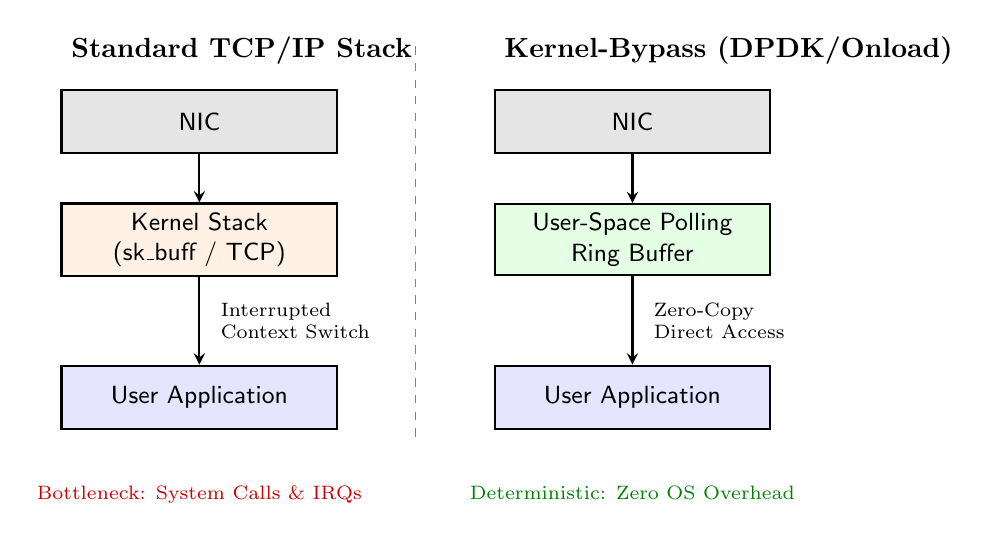
\begin{tikzpicture}[
        font=\sffamily\small,
        box/.style={rectangle, draw=black, thick, minimum width=3.5cm, minimum height=0.8cm, align=center},
        hw/.style={box, fill=gray!20},
        kernel/.style={box, fill=orange!10},
        user/.style={box, fill=blue!10},
        bypass/.style={box, fill=green!10},
        arrow/.style={->, thick, >=stealth}
    ]

    % Standard Path
    \node[anchor=west, font=\bfseries] at (0, 4.4) {Standard TCP/IP Stack};
    \node[hw] (std_nic) at (1.75, 3.5) {NIC};
    \node[kernel] (std_kern) at (1.75, 2.0) {Kernel Stack\\(sk\_buff / TCP)};
    \node[user] (std_app) at (1.75, 0) {User Application};
    \draw[arrow] (std_nic) -- (std_kern);
    \draw[arrow] (std_kern) -- node[midway, right=4pt, font=\scriptsize, align=left] {Interrupted\\Context Switch} (std_app);

    % Divider
    \draw[dashed, gray] (4.5, -0.5) -- (4.5, 4.5);

    % Bypass Path
    \node[anchor=west, font=\bfseries] at (5.5, 4.4) {Kernel-Bypass (DPDK/Onload)};
    \node[hw] (bp_nic) at (7.25, 3.5) {NIC};
    \node[bypass] (bp_poll) at (7.25, 2.0) {User-Space Polling\\Ring Buffer};
    \node[user] (bp_app) at (7.25, 0) {User Application};
    \draw[arrow] (bp_nic) -- (bp_poll);
    \draw[arrow] (bp_poll) -- node[midway, right=4pt, font=\scriptsize, align=left] {Zero-Copy\\Direct Access} (bp_app);

    % Highlights
    \node[anchor=north, font=\scriptsize, text=red!80!black] at (1.75, -1) {Bottleneck: System Calls \& IRQs};
    \node[anchor=north, font=\scriptsize, text=green!50!black] at (7.25, -1) {Deterministic: Zero OS Overhead};

    \end{tikzpicture}%
    }
    \caption{A comparison between the standard Linux networking stack and kernel-bypass technologies such as DPDK. While the standard stack requires the kernel to mediate packet delivery—introducing unpredictable context switches—kernel-bypass allows a user-space thread to poll the NIC hardware directly. This eliminates operating system overhead and provides the nanosecond-scale determinism required for HFT execution.}
    \label{fig:kernel_bypass_comparison}
\end{figure}
